\documentclass[letterpaper,12pt]{article}
\usepackage[margin=2cm]{geometry}
\usepackage[utf8]{inputenc}
\usepackage[english, spanish]{babel}
\usepackage{amsmath, amssymb}
\usepackage{tikz}
\usepackage{multicol}
\usetikzlibrary{automata,arrows}


%opening
\title{Autómatas y Lenguajes Formales, 2021-2 \\ Tarea 1}
\author{Oscar Andres Rosas Hernandez}
\date{\today}

\begin{document}

\maketitle

	
\begin{enumerate}
%%
%% Q1
\item (1.5 pts.) Sea $x$ una cadena, $x^R$ su reversa y $x^i$ la cadena concatenada consigo misma $i$ veces (por ejemplo: $(abc)^R = cba$ y $(abc)^2=abcabc$). Demuestre por inducción matemática que $(x^R)^i=(x^i)^R$. ({\bf Hint:} Use el hecho de que $(xy)^R=y^Rx^R$.)

%%
%% Q2
\item 
\begin{enumerate}
\item (0.5 pts.) Encuentre un lenguaje $L$ sobre el alfabeto $\Sigma = \{a,b\}$ que no sea $\{\varepsilon\}$ ni $\{a,b\}^*$ y satisfaga $L=L^*$.
\item (0.5 pts.) Dé un ejemplo de dos lenguajes $L_1$ y $L_2$ tales que $L_1^*\cup L_2^* \neq (L_1\cup L_2)^*$.
\item (0.5 pts.) Considere la siguiente definición recursiva para $L\subseteq\{a,b\}^*$: $b\in L$; $\forall w\in L$, $bw$, $wa$ y $aw$ están en $L$. Dé una definición no-recursiva para $L$ (por ejemplo, en español).
\end{enumerate}


%%
%% Q3 
\item (2 pts.) Suponga que $L\subseteq \{a,b\}^*$ se define como sigue:
   \begin{itemize}
   \item $\varepsilon \in L$,
   \item $\forall x,y\in L$, las cadenas $xy$, $axb$ y $bxa$  están en $L$.
   \end{itemize}
Demuestre que $L=L_{AB}$, el lenguaje de todas las cadenas $w\in\{a,b\}^*$ tales que $n_a(w)=n_b(w)$.

%%
%% Q4 
\item (2 pts.) Sea $M=(Q,\Sigma,\delta,q_0,F)$ un AFD. Sea $M_1=(Q,\Sigma,\delta,q_0,F_1)$ 
un AFD idéntico a $M$ excepto por el conjunto de estados finales, 
donde $F_1$ se define como el conjunto de estados 
$q\in Q$ para los cuales $\widehat{\delta}(q,z)\in F$ para alguna $z$. ¿Cuál es la relación entre el lenguaje aceptado por $M_1$ y el
 lenguaje aceptado por $M$? Justifique su respuesta. ({\bf Hint:} Use 
 el hecho de que $\widehat{\delta}(q, xy) = \widehat{\delta}(\widehat{\delta}(q, x), y)
$.\ )

Pues habra muchas relaciones entre los lenguajes que reconocen ambos automatas, uno de ellos, 
relativamente trivial es:

Sea $L_M$ el lenguaje que acepta $M$, $L_{M_1}$ el lenguaje que acepta $M_1$, entonces
$L_M \subseteq L_{M_1}$.

Esto se demuestra viendo que cualquier cadena que es aceptada por $M$ tambien lo es por $M_1$, dependiendo del 
automata particular puede que existan cadenas que solo acepte $M_1$.

Pero bueno, si una cadena $c$ es aceptada por $M$, entonces podemos decir que esta bien definida
la expresion $\widehat{\delta}(q_0, c)$, ahora podemos usar la idea que:
$c = c\epsilon$.

Entonces $\widehat{\delta}(q_0, c) = \widehat{\delta}(\widehat{\delta}(q_0, c), \epsilon)$.

Y recordemos que como esta cadena es aceptada por $M$ entonces podemos decir que:
$\widehat{\delta}(q_f, \epsilon)$, donde $q_f$ es un estado final, ahora,
podemos afirmar que $q_f \in F_1$ pues ya vimos que existe una transicion, esta: 
$\widehat{\delta}(q_f, \epsilon) = q_f \in F$.
Entonces $q_f \in F_1$, por lo tanto cualquier cadena aceptada por $L_M$ tambien la aceptara
$L_{M_1}$

%%
%% Q5
\item Describa informalmente el lenguaje reconocido por los siguientes Autómatas Finitos Deterministas (AFD):
\selectlanguage{english}
\begin{enumerate}
\item (1 pt.)
\begin{tikzpicture}[->,>=stealth',shorten >=1pt,%
auto,node distance=2.5cm,semithick,
inner sep=2pt,bend angle=45]

\node[initial,state, accepting, initial text=] (A)                               {$s_0$};
\node[state]         (B) [below right of=A]                       {$s_2$};
\node[state]         (C) [above right of=A]                       {$s_1$};
\node[state]         (D) [above right of=B]                       {$s_3$};

\path 
	(A) edge [bend left=15]		node {$ a $} (C)
    	  	edge [bend left=15]		node {$ b $} (B)
	(B) edge [bend left=15]      node {$ a $} (A)
		edge       			 	node [below right] {$ b $} (D)
	(C) edge [bend left=15]		node {$ b $} (A)
		edge  					node [above right] {$ a $} (D)
	(D) edge [loop right] 		node {$ a,b $} (D);

\end{tikzpicture}

\begin{align}
\{w\in \{a,b\}^* \, |\, w \mbox{ $(ab|ba)^*$ es decir, la concatenacion n veces de las cadenas $ab$ y $ba$ }\}
\end{align}

\item (1 pt.) 
\begin{tikzpicture}[->,>=stealth',shorten >=1pt,%
auto,node distance=2.5cm,semithick,
inner sep=2pt,bend angle=45]

\node[initial,state, accepting, initial text=] (A)                                {$s_0$};
\node[state]  				   (B) [right of=A]                   {$s_2$};
\node[state, accepting] 		   (C) [right of=B]                   {$s_1$};
\node[state]  		           (D) [below of=A]                   {$s_3$};

\path 
	(A) edge 		     	node {$ a $} (B)
    	  	edge	 				node {$ b $} (D)
	(B) edge [loop above]    node {$ a $} (B)
		edge [bend left=15]  node {$ b $} (C)
	(C) edge [bend left=15]  node {$ a $} (B)
		edge [loop above]	node {$ b $} (C)
	(D) edge [loop right] 	node {$ a,b $} (D);

\end{tikzpicture}

$\{w\in \{a,b\}^* \, |\, w \mbox{ Que empiece en $a$ y acabe en $b$}\}$



\end{enumerate}
\selectlanguage{spanish}

\newpage
%%
%% Q6
\item 
\begin{enumerate}
\item(1 pt.) Diseñe un Autómata Finito Determinista (AFD) que reconozca el lenguaje \linebreak $\{w\in \{a,b\}^* \, |\, w \mbox{ tiene como subcadenas a $ab$ y a $ba$.}\}$.
    \begin{figure}[ht]
    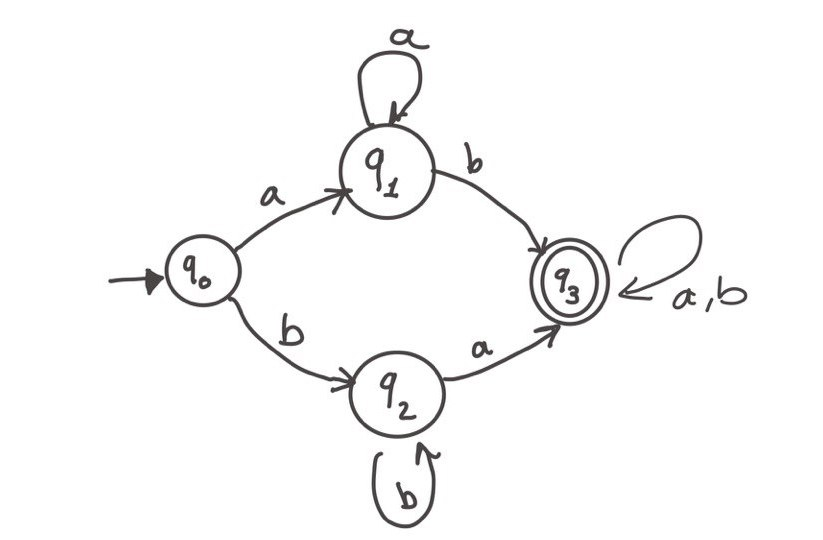
\includegraphics[width=0.45\textwidth]{Graphics/6n1}
  \end{figure}
  

\item (1 pt.) Diseñe un Autómata Finito Determinista (AFD) que reconozca el lenguaje \linebreak $\{w\in \{a,b\}^* \, |\, w \text{ contiene como subcadenas a $ab$ o a $bba$.}\}$.
    \begin{figure}[ht]
    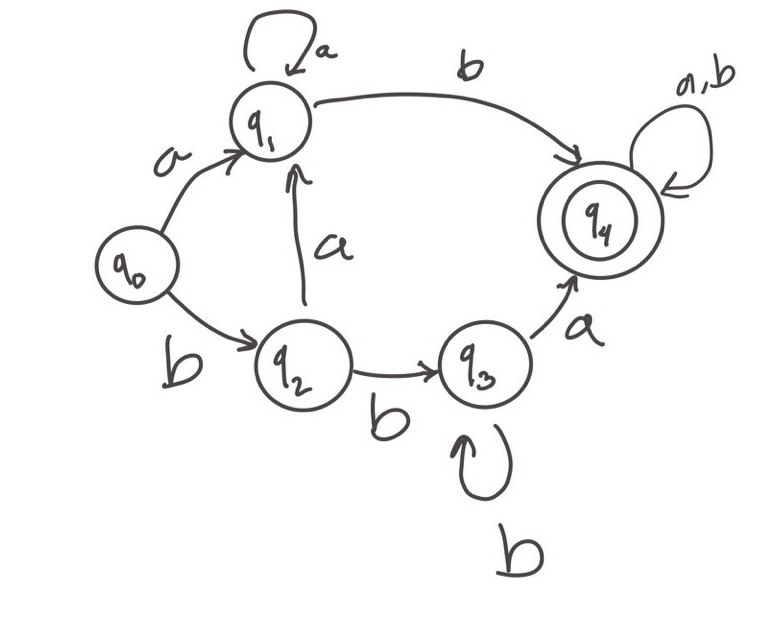
\includegraphics[width=0.45\textwidth]{Graphics/6n2}
  \end{figure}
  
\end{enumerate}

%% No more questions
\end{enumerate}

\end{document}
